\documentclass[12pt]{article}
\usepackage[utf8]{inputenc}
\usepackage[russian]{babel}
\usepackage{array}
\usepackage{makecell}
\usepackage{amsmath}
\usepackage{amssymb}
\usepackage{tikz}
\usepackage{float}

\usepackage{pgfplots}
\pgfplotsset{compat=1.18}

\usepackage{graphicx}
\graphicspath{ {./images/}}

\usepackage{geometry}
\geometry{
    left = 1cm,
    right = 2cm,
    top = 2cm,
    bottom = 2cm,
    bindingoffset = 1cm
}

\begin{document}
\begin{center}
    \hfill \break
    \hfill \break
    Санкт-Петербургский национальный исследовательский университет \\
    информационных технологий, механики и оптики \\
    \textbf{Учебный центр общей физики ФТФ} \\
    \vspace{12pt}
    \begin{tabular}[l]{m{0.2\textwidth} m{0.2\textwidth} m{0.4\textwidth}}
        \hline
        \textbf{Группа:} & Group & \textbf{К работе допущен:} \\
        \textbf{Студент:} & sltKaguya & \textbf{Работа выполнена:} \\
        \textbf{Преподаватель:} & Teacher & \textbf{Отчёт принят:}
    \end{tabular} \break
    \hfill \break
    \Large{\textbf{Рабочий протокол и отчёт по \\
    лабораторной работе №1.02}} \break
    
    \large{Изучение скольжения тележки по наклонной плоскости\\}\hfill
\end{center}

\begin{enumerate}
    \item Цели работы:
    \begin{enumerate}
        \item Измерение модуля ускорения свободного падения.
        \item Экспериментальная проверка эквивалентности гравитационной и инертной масс.
    \end{enumerate}

    \item Задачи, решаемые при выполнении работы:
    \begin{enumerate}
        \item 
    \end{enumerate}

    \item Объект исследования:
    \item Метод экспериментального исследования:
    \item Рабочие формулы и исходные данные:
    \item Измерительные приборы:
    \item Схема установки:\\
    Схема экспериментальной установки представлена на (Рис. \ref{pic:lab_set}).
    \begin{figure}[H]
        \centering
        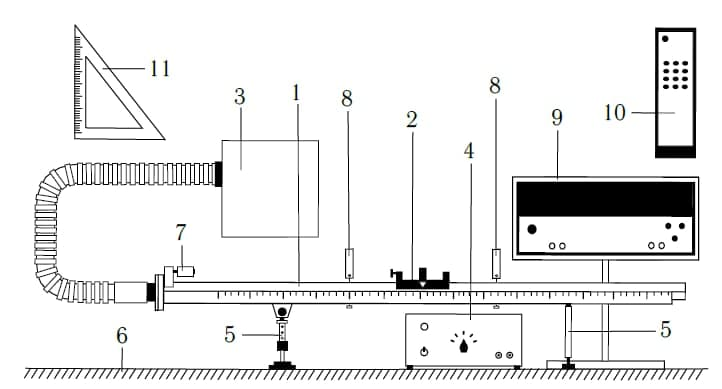
\includegraphics[scale=0.9]{laboratory_setup.jpg}
        \caption{Общий вид экспериментальной установки}
        \label{pic:lab_set}
    \end{figure}
    \begin{enumerate}
        \item[1.] Рельс с сантиметровой шкалой на лицевой стороне;
        \item[2.] Тележка;
        \item[3.] Воздушный насос;
        \item[4.] Источник питания насоса ВС 4-12;
        \item[5.] Опоры рельсы;
        \item[6.] Опорная плоскость (поверхность стола);
        \item[7.] Фиксирующий электромагнит;
        \item[8.] Оптические ворота;
        \item[9.] Цифровой измерительный прибор ПКЦ-3;
        \item[10.] Пульт дистанционного управления прибором ПКЦ-3;
        \item[11.] Линейка -- угольник.     
    \end{enumerate}
    По рельсу \textbf{1} скользит тележка \textbf{2}. Для уменьшения трения между поверхностями рельса и тележки создаётся воздушная подушка с помощью воздушного насоса \textbf{3}, подключенного к источнику питания \textbf{4}. Электрические провода, подключающие воздушный насос к источнику питания
    \item Результаты прямых измерений и их обработки:
    \item Расчёт результатов косвенных измерений:
    \item Расчёт погрешностей измерения:
    \item Графики: гистограмма и график плотности вероятности измеренного значения:
    \item Окончательные результаты:
    \item Выводы и анализы результатов работы:
    \item Дополнительные задания:
    \item Выполнение дополнительных заданий:
    \item Замечания преподавателя:
\end{enumerate}
\end{document}